--- layout: default ---

\section{Σύντομο βιογραφικό
σημείωμα}\label{ux3c3ux3cdux3bdux3c4ux3bfux3bcux3bf-ux3b2ux3b9ux3bfux3b3ux3c1ux3b1ux3c6ux3b9ux3baux3cc-ux3c3ux3b7ux3bcux3b5ux3afux3c9ux3bcux3b1}

\subsubsection{Προσωπικά
στοιχεία}\label{ux3c0ux3c1ux3bfux3c3ux3c9ux3c0ux3b9ux3baux3ac-ux3c3ux3c4ux3bfux3b9ux3c7ux3b5ux3afux3b1}

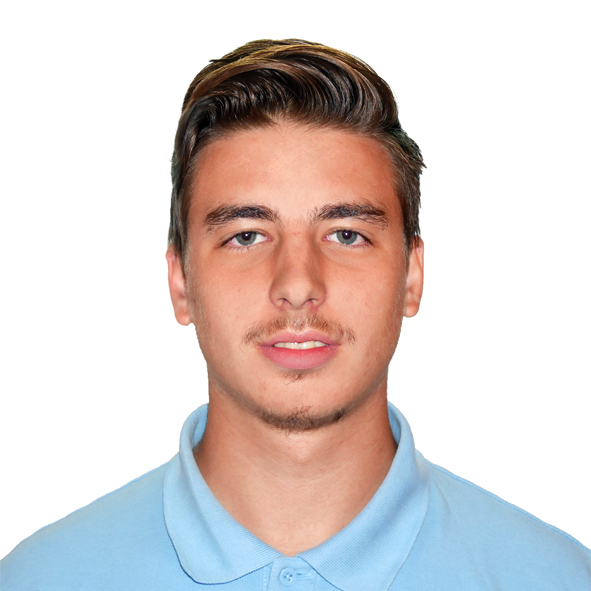
\includegraphics{\%7B\%7Bsite.baseurl\%7D\%7D/photo.jpg}

Ονοματεπώνυμο: Καλλιάρας Παύλος

Διεύθυνση: Ρήγα Φεραίου 42-44, Καρδίτσα

E-mail: paulosyeah@yahoo.gr

Τηλέφωνο: +306988614736

\subsubsection{Εκπαίδευση και
κατάρτιση}\label{ux3b5ux3baux3c0ux3b1ux3afux3b4ux3b5ux3c5ux3c3ux3b7-ux3baux3b1ux3b9-ux3baux3b1ux3c4ux3acux3c1ux3c4ux3b9ux3c3ux3b7}

2011: Συμμετοχή στον Πανελλήνιο Μαθητικό Καλλιτεχνικό Διαγωνισμό του
προγράμματος ``Οίκαδε''

2012 - 2013: Συμμετοχή του Γυμνασίου μου σε Ευρωπαϊκό πρόγραμμα
εθελοντισμού και έρευνας

2018: Αποφοίτηση από το 5ο Γενικό Λύκειο Καρδίτσας

2018 μέχρι σήμερα: Προπτυχιακές σπουδές Πληροφορικής
(\href{https://ionio.gr/}{Ιόνιο Πανεπιστήμιο})

2018: Συμμετοχή σε Local Hackday Event (Hackathon)

2019: Σεμινάριο για την κρυπτογραφία

\subsubsection{Εμπειρία}\label{ux3b5ux3bcux3c0ux3b5ux3b9ux3c1ux3afux3b1}

Βοηθός σε: Οικογενειακή αγροτική επιχείρηση

Γνώσεις: Πλήρη εξοικείωση με τον χειρισμό και συντήρηση αγροτικού
εξοπλισμού

Καλλιέργειες: Βαμβάκι, τριφύλλι, καλαμπόκι

\subsubsection{Δεξιότητες}\label{ux3b4ux3b5ux3beux3b9ux3ccux3c4ux3b7ux3c4ux3b5ux3c2}

Υπολογιστές: Χειρισμός Linux, Windows, εφαρμογές Office

Γενικές γνώσεις των γλωσσών: Python, C, C++, Java, HTML, CSS, SQL

Ξένες γλώσσες: Αγγλικά επιπέδου C2 (Edexcel)

Διπλώματα οδήγησης: Α' και Β' κατηγορίας

\subsubsection{Χόμπυ -
Ενδιαφέροντα}\label{ux3c7ux3ccux3bcux3c0ux3c5---ux3b5ux3bdux3b4ux3b9ux3b1ux3c6ux3adux3c1ux3bfux3bdux3c4ux3b1}

\begin{itemize}
\tightlist
\item
  Ποδηλασία
\item
  Χάρτες
\item
  Διαδρομές (ταξίδια)
\item
  Μεγάλα οχήματα
\end{itemize}
